% using Elseveir template per https://www.elsevier.com/authors/author-schemas/latex-instructions
% model paper: Dynamic effects of teacher turnover on the quality of instruction (2016)
%   Hanushek et al
%   from Economics of Education Review
% https://www.nber.org/papers/w22472

% secondary model paper: The effects of economic policy and political uncertainties on economic activities
% Gholipour, 2019
% https://www.sciencedirect.com/science/article/pii/S0275531918306081
\documentclass[review]{elsarticle}

\usepackage{amsmath}
\usepackage{lineno,hyperref}
\usepackage{booktabs}
\usepackage{graphicx}
\usepackage{hyperref}
\usepackage{siunitx}
\usepackage{tabularx}
\usepackage{threeparttable}  
\usepackage{tikz}

% ref: https://tex.stackexchange.com/questions/19390/how-do-you-download-packages-for-texworks-on-windows-7
% ref: https://tex.stackexchange.com/questions/47418/siunitx-specifying-custom-command-as-input-symbol
\newcommand{\sym}[1]{\rlap{#1}}

\bibliographystyle{elsarticle-num}
\graphicspath{{../alt-ed-survey/figures-and-tables}}
\journal{Journal of \LaTeX\ Templates}
\modulolinenumbers[5]
\sisetup{
    detect-mode,                        %%% not grammatical
    group-digits            = false ,   %%% not grammatical
    input-signs             = ,         %%% not grammatical
    input-symbols           = ()[]-+* , % specifying \sym here does not work  %%% not grammatical
    input-open-uncertainty  = ,         %%% not grammatical
    input-close-uncertainty = ,         %%% not grammatical
    table-align-text-post   = false     %%% not grammatical
}
\usetikzlibrary{calc,matrix}

\begin{document}
\begin{frontmatter}

    \title{
        The Impact of Employer Education Assistance on Enrollment
    }

    \author[mymainaddress]{John Vandivier} % \fnref{authorlinefootnote}}
    \address[mymainaddress]{4400 University Dr, Fairfax, VA 22030}
    \ead{jvandivi@masonlive.gmu.edu}

    \begin{abstract}
        % word count: 95
        % BHR maximum 100
        Policymakers incentivized higher education enrollment through the creation of Section 127 of the United States Internal Revenue Code.
        This policy provides a tax deduction to employers that provide financial assistance for employee education.
        This paper finds that before and after extensive correction, the policy fails to increase enrollment meaningfully.
        Evidence from 1992 through 2017 indicates adverse linear and total effects of interest.
        H-1B policy is explored as a correction variable and emerges as a comparatively preferred policy tool.
        Results are validated using vector autoregression (VAR), dynamic ordinary least squares (DOLS), and instrumental variable (IV) analysis.
    \end{abstract}

    \begin{keyword}
        tuition reimbursement, education economics, h-1b %%% not grammatical
        \MSC[2010] H4, I22, J32, J38
    \end{keyword}
\end{frontmatter}

\pagebreak
\linenumbers

\section{Introduction}
The passage of Public Law 95-600 in 1978 created Section 127\cite{plaw95_600_1978}.
Section 127 provides for a limited employer tax deduction for the transfer of money to an employee for educational purposes.
This paper tests the hypothesis that the effect of Section 127 employer assistance on total university enrollment is positive.
Results show that employer assistance has a positive marginal effect on enrollment and negative linear and total effects.
Evidence indicates that H-1B visa policy is a comparatively effective policy instrument for enrollment,
national student loan debt, and the price of education.

% address unclear research question
% but I already had a hypothesis is it not weird to have both?
% use hanushek trick to add the question in a summary line
% ref: https://pubs.aeaweb.org/doi/pdfplus/10.1257/jel.46.3.607
Total enrollment is one of a few policy concerns related to Section 127.
The paper concludes by asking whether the results observed represent policy success.
In summary, how do Section 127 results over time relate to its policy goals?
This paper finds that Section 127 has achieved partial success,
but several changes are advisable.

Figure \ref{fig:intro_enroll_assistance} illustrates university enrollment over time
and the real maximum deductible amount for Section 127 educational assistance.
% Here, education-specific inflation informs the real assistance limit.
This paper hypothesizes that the apparent inverse relation is a superficial result of variable omission.
Analysis in this paper controls extensively for dynamic policy and economic variation.
The use of multiple specifications ensures the robustness of findings.
In one specification, vector autoregression (VAR) provides evidence on utility as a policy instrument.

\begin{figure}[h!]
    \centering
    \caption{Enrollment and Real Assistance Over Time}
    \begin{tikzpicture}[element/.style={minimum width=1.75cm, minimum height=0.85cm}]
        \node (n1) {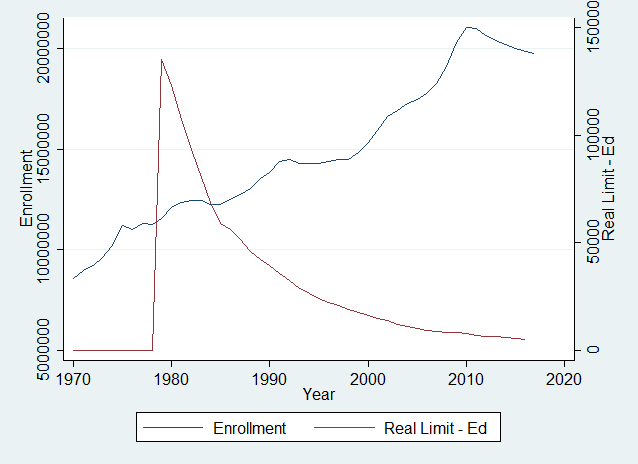
\includegraphics[width=1\textwidth]{./figures-and-tables/intro-enroll-over-time-and-assistance-limit.png}};
    \end{tikzpicture}
    \label{fig:intro_enroll_assistance}
\end{figure}

\section{Methodology}

This paper broadly explores Section 127 effects in comparison to its policy goals.
The focus of this broad conversation is the identification of the policy effect on total enrollment.
This identification proceeds from statistical analysis across multiple specifications.
This paper operationalizes total enrollment as a representation of one of the original Section 127 policy goals.

% SHRM assessed only a single year, 2008. Shows Section 127 is mostly a Master's degree tool rn.
The Society for Human Resource Management (SHRM) \cite{jones_2010} identifies three original policy goals for the passage of Section 127.
% Operationalization of total enrollment as a success measure is derived from the third policy goal.
The third policy goal is to incentivize upward mobility by providing funds for higher education.
As a result, this paper takes total enrollment as the dependent variable.

Specifications begin with an ordinary least squares (OLS) investigation.
Finding significant time effects justifies and motivates further analysis.
Dynamic ordinary least squares replicates the importance of time effects,
and also addresses concerns on potential autocorrelation.
Finally, a vector autoregression indicates that certain policy changes
are candidate policy instruments.

% The failure of several simple theories to successfully explain the observation of enrollment slowdown in the late 1970s and 1980s further motivates the present study.

% \subsection{Simple Supply-Side Explanations}
% One hypothesis is that there is an adjustment period between the creation of Section 127 and widespread employer provision of the newly deductible benefit.
% Allowing for a 3 or 5 year lag around the passage of Public Law 95-600 fails to harmonize observed enrollment slowdown with the expected increase to demand.
% Across the eight five-year periods from 1970 to 2010, the five-year public enrollment growth rate was above 9 percent half of the time.
% Two of the four low-growth intervals occurred immediately after the 1978 creation of Section 127.
% The period just prior, from 1970-1975, saw the highest growth in enrollment across those eight periods.

% Surveys of employers provide further data on employer provision of educational assistance over time.
% Cappelli identifies three employer surveys from 1992 and 1993, which indicate that at least 86 percent of surveyed employers provided educational assistance\cite{cappelli2004employers}.
% These early surveys consist of samples of convenience.
% Nevertheless, further considerations lead Cappelli to conclude that a substantial majority of employers offered such plans over his period of analysis from about 1990 to 2004.
% The provision of this kind of benefit remains common in later years.
% In 2013, SHRM reported that 61 percent of employers offer tuition assistance\cite{cherry2014rejuvenating}.
% In 2017, World at Work found that 85 percent of employers offered such a benefit,
% with another 7 percent offering non-reimbursement tuition assistance, such as upfront tuition discounts\cite{talentculture_2018}.
% In summary, the simplistic hypothesis of lagged or bottlenecked employer support for Section 127 fails to solve the problem.

% \subsection{Simple Demand-Side Explanations}
% A simple regression of real employer assistance on enrollment may yield a significant negative correlation wholly due to consumer effects.
% The factual claim of decreasing market demand is consistent with observation, but it began before the passage of Section 127.
% Falling average tuition and fees are observed for all institutions from 1972 to 1980.
% The college-age enrollment percent does not increase substantially from 1970 to 1980.
% Higher education prices increase after 1980, as do the college-age enrollment percentage and total enrollment.

% Because the decline in demand predates the passage of Section 127, the cause of decline must be located elsewhere, at least in part.
% Simplistic demand-side identification of the effects of employer assistance fails due to omitted variable bias.
% Important omitted variables include controls for inflation, the price of education, and relevant policy changes.
% Immigration, veteran education, and federal lending policy undergo fundamental changes in proximity to 1978 and in years later.
% Sufficient identification of the effect of Section 127 must account for changes in these variables over time.

\section{Empirical Model}

This paper takes multiple steps to ensure robustness and analytical completeness.
The final results are consistent across three empirical specifications.
In addition to the variable of interest, this paper tests two other left-hand variables.
Testing these two secondary dependent variables of interest improves confidence in the theoretical and applied soundness of the conclusion.

Total postsecondary enrollment in the United States is the dependent variable.
The Section 127 policy effect is the right-hand parameter of interest in the first two specifications.
Equation \ref{eq1} is the first specification of interest. This model is an ordinary least squares model.
Here, $\alpha$ is a $1*k$ vector of coefficients,
and $V$ is a $k*1$ vector of annually observed independent variables.

% time-invarient coefficients.
% all betas are linear coefficients of their respective independent variables
% nonlinear effects are capture with exponential transforms as distinct independent variables.
% OLS
\begin{equation}
    % alternatively, longer-form:
    % Y_t = \beta_1X_{1t}+\beta_2X_2...+\beta_kX_k+e
    Y_t = \alpha{V_{t}}+u_t
    \label{eq1}
\end{equation}

Policy variables exist for federal lending policy, veteran education benefits, and H-1 Visa policy.
Two additional non-policy variables include time, in years,
and the real price of university tuition plus mandatory fees.

Equation \ref{eq2} describes the next specification.
This model follows the Anderson–Hsiao pattern\cite{anderson1981estimation} with the lagged variable of interest as an instrument.
This specification investigates concerns of potential endogeneity in the dependent variable.
It is both an instrumental variable model and also a dynamic ordinary least squares (DOLS) model.

% DOLS
% ref: http://www3.grips.ac.jp/~yamanota/Lecture%20Note%208%20to%2010%202SLS%20&%20others.pdf
% could be important to acknowledge that "you must be aware that the standard errors from the two-step procedure
%   are incorrect, usually smaller than the correct ones" per supra
%   but in our case beta of interest isn't importantly different between preferred DOLS and non-IV transform
% ref: https://www-jstor-org.mutex.gmu.edu/stable/2287517?seq=2#metadata_info_tab_contents
% ref: preferred dols model from analysis-9-dols-reg-table.do
% note: Dickey-Fuller test for the presence of a unit root
%   would be an alternative, or additional, way to check for dependent var endogeneity
\begin{subequations}
    \begin{equation}
        \Delta{Y_t} = \beta{W_{t}}+B{z_t}+e_t
        \label{eq2}
    \end{equation}
    \begin{equation}
        z_t = \delta{W_{t}}+D{Y_{t-2}}+g_t
        % I think this is a better derivation but I'm not sure if it's completely correct:
        % z = \hat{Y}_{t-1} = \delta{W_{t}}+D{Y_{t-2}}+g_t
        \label{eq3}
    \end{equation}
\end{subequations}

Here, $\beta$ is a $1*l$ vector of coefficients,
and $W$ is an $l*1$ vector of annually observed independent variables.
$z$ is the instrument, and it is a projection of lagged enrollment derived from twice-lagged enrollment.
Equation \ref{eq3} explicitly derives $z$.
% B is the particular explanatory coefficient for $z$.
% lowkey B assumes invariance over time but let's not talk about it

$l$ is a transformation of $k$ from Equation \ref{eq1}.
$l$ contains five variations of each variable in $k$.
The first variation is the non-transformed value.
The other variations include the first and second lags and differences for each variable in $k$.
% In Equation \ref{eq3},
% $\delta$, $D$, and $g$ fill modelling roles analgous to $\beta$,
% $B$, and $e$ from Equation \ref{eq2}.

The third specification is a vector autoregression (VAR) model.
Six related models follow the general reduced form
described in Equation \ref{eq:applied_naiive_var}.
This first model following this functional form is a two-variable case.
This first model is similar to the previous non-VAR
specifications because it identifies the effect of
real employer assistance on total enrollment.
A second model follows the same form,
but the independent variable is H-1B visa issuance,
instead of Section 127 assistance.

\begin{subequations}
    \begin{equation}
        v_t = \alpha_0 + \alpha_1{v_{t-1}} + \alpha_2{v_{t-2}} + ... + \alpha_i{v_{t-i}} + u_t
        \label{eq:univariate_var}
    \end{equation}
    \begin{equation}
        V_t = \alpha_0 + \alpha_1{v_{1, t-1}} + \alpha_2{v_{2, t-1}} + ... + \alpha_{ik-1}{v_{k-1, t-i}} + \alpha_{ik}{v_{k, t-i}} + u_t
        \label{eq:naiive_multi_var}
    \end{equation}
    \begin{equation}
        Y_t = \sigma_k{V_{kt}}+e_t
        \label{eq:applied_naiive_var}
    \end{equation}
\end{subequations}
% TODO: maybe use stata built-in Granger causality Wald tests

Equation \ref{eq:univariate_var} is a univariate autoregression.
Dependent and independent variables are uniformly represented by $v_t$.
An ordinary least squares function of $i$ lags explains the current-period value of the variable in the univariate regression.
Equation \ref{eq:naiive_multi_var} extends this operation to $k$ variables.
Notice that $V_t$ is not a collection of univariate $v_t$.
Instead, it is a $k*k$ vector, a constant, and an error term.

Equation \ref{eq:applied_naiive_var}
obtains $V_t$ as specified in Equation \ref{eq:univariate_var}
for all variables in $k$,
then fits an ordinary least squares model across $V_kt$ to explain the current-period dependent variable, $Y_t$.
Section 127 effects turn out to be insignificant in the specification described by Equation \ref{eq:applied_naiive_var},
but H-1B effects are significant.
As a result, all four remaining VAR equations use H-1B issuance as the independent variable.

% another good article from david, other than cited: https://blog.stata.com/2016/08/09/vector-autoregressions-in-stata/
% Lucas critique of VAR https://ocw.mit.edu/courses/economics/14-384-time-series-analysis-fall-2013/lecture-notes/MIT14_384F13_lec12and13.pdf
Two of the four remaining models are three-variable extensions of the prior specification.
These two models extend Equation \ref{eq:applied_naiive_var} by adding a second stage response.
In the first case, the second-order response is federal student loan debt.
In the second case, the second-order response is the price of higher education.
David Schenk suggests Cholesky decomposition as a method of generating an ordered impulse-response function from a VAR\cite{schenck_2016}.
Equations \ref{eq:make_structural_shocks} and \ref{eq:link_covariance_error} describe Cholesky identification.

\begin{subequations}
    \begin{equation}
        e_t = Bu_t
        \label{eq:make_structural_shocks}
    \end{equation}
    \begin{equation}
        \Sigma = E(e_t e_t')
        = E(Bu_tu_t'B')
        = B E(u_t u_t') B'
        = B B'
        \label{eq:link_covariance_error}
    \end{equation}
\end{subequations}

% I think $u_t$ is a vector and not a matrix right...?
The left-hand error term in Equation \ref{eq:make_structural_shocks}, $e_t$,
is the same as in Equation \ref{eq:applied_naiive_var}.
The right-hand of Equation \ref{eq:make_structural_shocks} defines $B$,
which is the coefficient matrix for $u_t$.
Structural, or uncorrelated, errors are defined as $u_t$.
Endogenous error in $B$ allows us to estimate the effects of arbitrary innovation in some variable in $V_k$.

The reduced form $BB'$ in Equation \ref{eq:link_covariance_error} matches many matrices.
There does exist a unique lower-triangle matrix that satisfies
the equality statement with $\Sigma$, the covariance matrix of the errors.
% Selecting the lower-triangle solution is isomorphic to stipulating a causal direction of effect on the variables in the VAR.
Selecting the lower-triangle represents analyst stipulation of the order in which effects are realized.
The order imposed is called a Cholesky ordering.
This paper selects theoretically-grounded Cholesky orderings.
% Measures of the fitness of the resulting models are considered evidence about Granger causality.

The last two models in the six-model VAR family are also simple two-factor VAR models.
These models test the hypothesis that enrollment effects are extraneous
to the effects of H-1B policy on student loans and the price of higher education.
The form of these models follows the specification in Equation \ref{eq:applied_naiive_var},
but the independent and response variables are different.
H-1B issuance is the independent variable.
The response variable is federal student loan debt in one case.
The price of higher education is the response variable in the other case.

\section{Description of Data}

% Ordinary least squares analysis begins with eight independent variables.
Models in this paper use a subset of nine high-level variables.
Enrollment figures for all degree-granting postsecondary institutions in the United States
are provided by the National Center for Education Statistics (NCES)\cite{nces_2019}.
Enrollment figures are for the fall semester of the school year.
% The values that NCES provides for years after 2018 are projections.
% This study does not use those projected values.
% total enrollment: https://nces.ed.gov/programs/digest/d18/tables/dt18_303.10.asp

For the same group of institutions,
NCES elsewhere provides data about average tuition and required fees\cite{nces_2017}.
This study uses price information for full-time undergraduate students.
% why? 1) most students are full-time undergrads, and,
% 2) we already know how the policy affects grad students. we want to know how it effects undergrads
Prices do not include the cost of room and board.
Cost information exists through the year 2016
% NCES provides nominal values and values adjusted for the consumer price index (CPI) for tuition.
Cost information reflects real prices.
2016 is the base year for Consumer Price Index (CPI) adjustment.
% https://nces.ed.gov/programs/digest/d17/tables/dt17_330.10.asp

% Nominal Section 127 limits are a matter of public law.
Section 127 took effect on January 1, 1979, with a nominal assistance limit of 5,000 dollars\cite{plaw95_600_1978}.
In October 1986, Pub. L. 99–514 increased the nominal assistance limit to 5,250 dollars\cite{plaw99_514_1986}.
Nominal limits are adjusted for education-specific inflation using NCES price data.
The real employer assistance limit is the primary explanatory variable of interest to this study.

Section 127 was renewed several times over the years.
A dummy variable exists for a considerable change realized in 2013.
In that year, the employer assistance deduction became permanent.
Personal Consumption Expenditures (PCE) data is a measure of inflation provided by the U.S. Bureau of Economic Analysis (BEA)\cite{bea_2020}.
PCE is a fourth independent variable.
% Broad representation of dynamic price effects in the economy is achieved
% by having seperate variables for general inflation and education-specific inflation.
% Combining nominal assistance over time with CPI and education-specific inflation data yields two real measures of inflation.

% Why nominal loan limit? well, real is worth testing but we already have inflation variables
Stafford loan data is another critical high-level component of the analysis.
Stafford loan limits impact the supply of loanable funds, which indirectly modifies demand for education.
Stafford data also broadly proxies non-military federal student aid policy.
Stafford loans technically decompose into two lower-level factors.
The first is the nominal loan limit for undergraduates.
The second variable is a dummy variable.
The dummy variable indicates whether the undergraduate loan limit is the combined limit for undergraduate and graduate loans.
A policy change in 1993 grouped these limits.
FinAid provides the Stafford loan data used in this study\cite{finaid_2020}.

% H-1 family of factors are collectively variable #5
Visa policy is the sixth high-level variable.
The number of H-1B visas issued each year is an essential variable in this study.
The Immigration Act of 1990 decomposed the existing H-1 visa into distinct H-1A and H-1B categories.
Later legislation established the H-1B1, H-1C, and many other visa classifications, but these are mostly inapplicable to the present research.
The H-1B visa is most relevant for this study because it relates explicitly to the undergraduate degree.
The Immigration Act of 1990 makes available the H-1B classification for specialized workers, or workers in a specialty occupation.
That legislation formally defines a specialty occupation as "an occupation that requires...attainment of a bachelor's or higher degree..."
The period of analysis for this study is constrained to begin with the advent of H-1B data in 1990.
As earlier mentioned, tuition data constraints the end of the analysis to 2016.

H-1 visas are a subgroup of nonimmigrant visas.
The Bureau of Consular Affairs provides nonimmigrant visa award data by classification
from 1987 to 2019\cite{bureauof_2020}.
This paper exclusively uses the most relevant H-1B visa award numbers,
but reanalysis with other visa classifications could yield statistically significant findings.
The prior H-1 visa was also a merit worker visa, but it had no formal definition of merit.
It is plausible that the college-educated effect informally existed before the 1990 legislation.
One might also find small but significant effects by looking into visas outside the H-1 family.
Besides the number of actual visa awards,
an analyst could look for visa cap effects or visa policy state effects.
For example, the Pew Research Center notes that the American Competitiveness in the 21st Century Act of 2000 exempts certain entities from the H-1B cap\cite{ruiz2017key}.
% ref: https://en.wikipedia.org/wiki/H-1B_visa#H-1B_visas_issued_per_year
% more state variable food https://redbus2us.com/h1b-visa-total-cap-history-from-1990-to-current-year/
% 1952 allows unlimited merit immigration, 1990 there is a quota and degree requirement added to H-1B: https://en.wikipedia.org/wiki/H-1B_visa#Immigration_Act_of_1990
% A crackdown in 2017: https://www.investopedia.com/news/impact-trumps-h1b-visa-crackdown-5-charts/
% other policies for policy state analysis:
%   https://en.wikipedia.org/wiki/Legal_Immigration_Family_Equity_Act#V_visa
%   not sure it's relevant - https://en.wikipedia.org/wiki/Immigration_Reform_and_Control_Act_of_1986
%   https://en.wikipedia.org/wiki/H-1B_Visa_Reform_Act_of_2004
%   1986 we get h-2a and h-2b https://www.uscis.gov/ilink/docView/AFM/HTML/AFM/0-0-0-1/0-0-0-13593/0-0-0-13614.html
%   more 1986 context https://www.vox.com/2014/9/3/18080710/immigration-immigrants-reform-us
%   various visa info https://uk.usembassy.gov/visas/temporary-employment/petition-based-visas/
% 
% Open SE questions looking for more data:
% 1) https://politics.stackexchange.com/questions/52279/us-pre-1987-visa-issue-data
% 2)
% 
% Open Tweet looking for more data:
% https://twitter.com/JohnVandivier/status/1243975718649974786
% apparantly official response via twitter...cite if you dare: https://twitter.com/TravelGov/status/1243985245382283266
% they daring me: https://academia.stackexchange.com/questions/119549/can-a-tweet-be-added-to-graduate-research-proposal
% "with the caveat of ambiguous language,
%   the State Department appears to confirm tha pre-1987 data is currently digitally unavailable,
%   and perhaps permentantly unrecorded even offline."

Actual federal loans stand in contrast to loan limits, which are represented by the Stafford loan limit variable.
Loan limits are a policy choice, but after correcting for loan limits,
the actual amount of loans made primarily represents a demand effect.
As such, we would not want to correct for actual loans.
That would wipe out the effect of interest,
which is the demand effect attributable to various policies,
and Section 127 employer educational assistance in particular.

Loan data generates results as a left-hand variable of secondary interest, rather than as an independent variable.
The variable I use in this regard is total federal undergraduate loans.
College Board provides loan data.
College Board also gives the additional context in a report which is related to the loan data\cite{cb_excel_2019}.
The additional context suggests that an analysis that decomposes federal loans by type could yield preferred statistical results\cite{cb_trends_2019}.
% actual undergrad loans awarded since 1990 in the excel at https://research.collegeboard.org/trends/student-aid
% My variable `Total UG Federal Loans` adapted from CB xlsx worksheet `Table 2_UG`

% Note: arguably, we don't need to discuss veteran education benefits at all bc they aren't significant in the new analysis.
% Changes to veteran education benefits are also a matter of public law.
The final subset of data describes veteran education benefits policy.
Each year in the data set is associated with some veteran education policy.
Veteran policy effects are a high-level variable which technically decompose into seven dummy variables.
A series of seven dummy variables capture veteran education policy effects.
The seven variables cover the period from 1944 to 2021.
The Servicemen's Readjustment Act of 1944 is also called the G.I. Bill.
The original bill expired in 1956\cite{glass_2010}.
The period from 1944 to 1956 is positively associated with the first dummy variable.

The Veterans Educational Assistance Program (VEAP) passed in 1981\cite{veteransaffairs_2017}.
The third period of interest ends in 1984 with the enactment of the Montgomery GI Bill\cite{powers_2018}.
The fourth period of interest ends in 2009 with the Post-9/11 GI Bill.
Finally, many benefits from the Forever GI Bill became effective in 2018,
with additional provisions taking effect in 2020 and 2022\cite{veteransaffairs_2020}.

Because of time sample constraints on other variables,
there is only a single variation in veteran education benefits during the period of analysis.
This is the enactment of the Post-9/11 GI Bill in 2009.
% This factor does prove to be significant in the preferred model.

Recent changes in veteran education benefits and in Section 127
represent critical caveats for any attempt at forecasting outside of the period of study.
As mentioned, the Forever GI Bill lays out several important changes in veteran benefits in the years to come.
Under the CARES Act, Section 127 was amended to provide a new benefit on a temporary basis\cite{schiavo_2020}.
The new benefit is that employers may assist employees in paying down existing student loan debt,
rather than only paying for new expenses, in a tax deductable way.
Under current law, the CARES Act changes to employer assistance will apply only during the year 2020.

% GI Bill accounting https://en.wikipedia.org/wiki/G.I._Bill#Chapter_30_(Montgomery_GI_Bill)
% Variable implemented as categorical
% [state A] original bill was 1944-1984
% [state B] VEAP established 1981 https://www.benefits.va.gov/gibill/veap.asp
% [state C] Montgomery GI went into effect 1984
% [state D] Post-9/11 GI Bill went into effect for 2009 school year https://www.thebalancecareers.com/gi-bill-for-the-21st-century-3347143
% [state E] Forever GI bill rolls out new benefits starting in 2018 https://rebootcamp.militarytimes.com/education-transition/education/2017/08/16/trump-signed-the-forever-gi-bill-here-are-11-things-you-should-know/

\section{Results}

% note: per editor feedback, don't admit that selected tuition measure is based on horse racing
% I stand by the fact that horse racing is the good, honest, and objective selection process
% Replacing tuition with PCE and education-deflated employer assistance in model 2 identifies the latter
% with significance at the 0.1 level and also improves the overall explanatory power of the model.
% Real employer education assistance, which is solely corrected for the price of education,
% is eventually preferred to the multiple-deflated measure.
% This makes the education-deflated real employer assistance limit the preferred Section 127 variable.
% After deciding on this variable as the preferred measure,

\subsection{Multiple Regression Results}
% Perhaps undergraduate enrollment is more relevant than total enrollment, but that is out of scope of this paper.
% The key independent variable is the real value of Section 127 assistance.
The prior description of data notes seven indepenent variables and two dependent variables.
Total university enrollment is the primary dependent variable.
Initial regression analysis involves ordinary least squares regression of all seven independent variables
on the primary dependent variable,
plus a variable for time.

Results for the initial regression model are described as Model 1 within Table \ref{tab:table_multiple}.
This table presents selected variables, where selected variables are significant in at least two specifications.
Section 127, inflation, and time effects were the most important variables in Model 1 (p < 0.000).
Linear and nonlinear employer assistance effects were significant.
A dummy variable which represented whether the employer deduction was temporary or permanent was also significant.

Linear and nonlinear visa policy effects were also highly significant (0.001 < p < 0.05).
Tuition and the interaction between Section 127 and visa policy were notably insignificant.
Veteran education benefits and Stafford variables were also insignificant.

\begin{table}
    \caption{Table of Multiple Regression on Enrollment, Selected Variables}
    \resizebox{\columnwidth}{!}{
        
\begin{tabular}{l*{4}{c}}
    \toprule
                             &\multicolumn{1}{c}{(1)}&\multicolumn{1}{c}{(2)}&\multicolumn{1}{c}{(3)}&\multicolumn{1}{c}{(4)}\\
                             &\multicolumn{1}{c}{Enrollment}&\multicolumn{1}{c}{Enrollment}&\multicolumn{1}{c}{Enrollment}&\multicolumn{1}{c}{Enrollment}\\
    \midrule
    Montgomery GI            &  -1058516.3\sym{*}  &  -1079802.6\sym{*}  &  -1075752.6\sym{***}&   -960383.2\sym{*}  \\
                             &  (419485.4)         &  (409292.0)         &  (266842.9)         &  (353349.0)         \\
    \addlinespace
    Real Limit - Ed and PCE  &                     &      -965.9         &                     &                     \\
                             &                     &     (519.8)         &                     &                     \\
    \addlinespace
    Real Limit - Ed          &      1162.1\sym{***}&      1231.5\sym{***}&                     &      -441.6         \\
                             &     (217.1)         &     (226.0)         &                     &     (309.2)         \\
    \addlinespace
    Real Limit - Ed$^2$        &                     &                     &      0.0353\sym{***}&      0.0591\sym{***}\\
                             &                     &                     &   (0.00871)         &   (0.00730)         \\
    \addlinespace
    Real Limit - Ed$^3$        &                     &                     &-0.000000475\sym{**} &-0.000000830\sym{***}\\
                             &                     &                     &(0.000000156)         &  (9.79e-08)         \\
    \addlinespace
    Tuition CPI              &       742.2         &                     &                     &                     \\
                             &     (463.8)         &                     &                     &                     \\
    \addlinespace
    H-1 Visa                 &      -78.20\sym{**} &      -77.02\sym{**} &      -26.46         &                     \\
                             &     (22.84)         &     (22.14)         &     (19.38)         &                     \\
    \addlinespace
    H-1B Visa                &      -46.67         &      -50.77         &                     &      -17.31\sym{*}  \\
                             &     (25.16)         &     (24.96)         &                     &     (7.763)         \\
    \addlinespace
    H-1B$^2$                   &    0.000936\sym{*}  &    0.000994\sym{*}  &   0.0000856         &   0.0000427         \\
                             &  (0.000406)         &  (0.000402)         & (0.0000680)         & (0.0000339)         \\
    \addlinespace
    H-1 Non-H-1B             &       127.3\sym{**} &       123.8\sym{**} &       52.89         &                     \\
                             &     (39.18)         &     (37.78)         &     (32.95)         &                     \\
    \addlinespace
    Year                     & 416886180.7\sym{**} & 409416696.8\sym{**} & 236525780.3\sym{***}& 247765777.0\sym{***}\\
                             &(123581479.5)         &(113020808.8)         &(27200513.3)         &(32364317.1)         \\
    \addlinespace
    Year$^2$                   &   -103662.0\sym{**} &   -101789.9\sym{**} &    -58751.0\sym{***}&    -61552.8\sym{***}\\
                             &   (30771.6)         &   (28136.8)         &    (6755.8)         &    (8021.7)         \\
    \midrule
    R-sqr                    &      0.9973         &      0.9975         &      0.9970         &      0.9965         \\
    \bottomrule
    \multicolumn{5}{l}{\footnotesize Standard errors in parentheses}\\
    \multicolumn{5}{l}{\footnotesize \sym{*} \(p<0.05\), \sym{**} \(p<0.01\), \sym{***} \(p<0.001\)}\\
    \end{tabular}
    }
    \label{tab:table_multiple}
\end{table}

Model 2 is obtained by removing insignificant variables from Model 1.
The importance of time in this analysis motivates further analysis using specifications that are explicitly dynamic.

\subsection{Dynamic Ordinary Least Squares Results}
% ref: analysis-3-dynamic-ols.do

Models 3 and 4 from Table \ref{tab:table_multiple} are dynamic ordinary least squares (DOLS) models.
These models are specially created to address concerns about potential autocorrelation using an Anderson-Hsiao adjustment\cite{anderson1981estimation}.
DOLS models also benefit marginal analysis by decomposing within-period and between-period marginal effects.
Model 3 is generated by applying an Anderson-Hsiao adjustment to Model 2.
In addition, first and second lags and differences were checked for each significant variable in Model 2.
Model 4 is the result of trimming insignificant variables from Model 3.

% Does angerson-hsiao really work tho?
% ref: https://stats.stackexchange.com/questions/464481/why-does-the-anderson-hsiao-adjustment-pick-the-twice-lagged-first-difference
% ref: https://en.wikipedia.org/wiki/Arellano%E2%80%93Bond_estimator
The Anderson-Hsiao adjustment involves three changes that allow an analyst to address actual or potential autocorrelation in the dependent variable.
The first step is to replace the dependent variable with its first difference.
The second change is a refinement in specification.
Models 3 and 4 are a special case of DOLS multiple regression because they are also instrumental variable models.
The third step in the Anderson-Hsiao adjustment is to pick a particular instrumental variable.
This particular instrument is often called the Anderson-Hsiao estimator.
The Anderson-Hsiao estimator is the twice lagged first difference of the dependent variable.
% The result of these three specification changes is that overlapping periods are removed from the model.
% This addresses concerns of potential autocorrelation over time.



% below only true if factors are robust across specifications, else need a model 5.
Model 4 is the preferred least squares model.

\begin{table}
    \caption{Table of DOLS Regression on Total Enrollment, Selected Variables}
    \begin{tabularx}{\textwidth}{X}
        \centering
        
\begin{tabular}{l*{2}{c}}
    \toprule
                             &\multicolumn{1}{c}{5}&\multicolumn{1}{c}{6}\\
    \midrule
    H-1B$^2$                   &  -4.217e-06        &   7.578e-04\sym{++}\\
                             & (5.768e-05)        & (3.354e-04)        \\
    \addlinespace
    H-1B$^3$                   &                    &  -2.086e-09\sym{++}\\
                             &                    & (9.547e-10)        \\
    \addlinespace
    Real Limit - Ed          &   3.359e+02        &  -2.202e+02\sym{+} \\
                             & (5.214e+02)        & (1.014e+02)        \\
    \addlinespace
    Real Limit - Ed$^2$        &  -4.256e-04        &   5.406e-03\sym{++}\\
                             & (1.294e-02)        & (2.026e-03)        \\
    \addlinespace
    Year$^2$                   &  -2.064e+04        &  -5.706e+01\sym{*} \\
                             & (1.633e+04)        & (1.489e+01)        \\
    \midrule
    R-sqr                    &      0.5172        &      0.9252        \\
    \bottomrule
    \multicolumn{3}{l}{\footnotesize Standard errors in parentheses}\\
    \multicolumn{3}{l}{\footnotesize \sym{+} \(p<0.10\), \sym{++} \(p<0.05\), \sym{*} \(p<.01\), \sym{**} \(p<.001\)}\\
    \end{tabular}
    \end{tabularx}
    \label{tab:table_dols}
\end{table}

The preferred dynamic OLS model obtains an adjusted r-squared of about 0.85.
In contrast, the simple adjustment to the preferred multiple regression
obtains an adjusted r-squared of about 0.26.
A surprising result is that the Anderson-Hsiao estimator is insignificant
across various specifications, including the preferred DOLS model (p = 0.51).
Time effects are independently significant in the model.
These results indicate the absence of autocorrelation.
Instead, time efficiently proxies unobserved independent effects.

While the Anderson-Hsiao estimator is insignificant,
dropping that variable and running an ordinary regression reduces adjusted r-squared to 0.82,
but all independent factors retain significance.
This demonstrates comparative model robustness over the preferred multiple regression.
For this reason, the preferred DOLS model, with or without instrumentation,
is preferred to the preferred multiple regression identified as
model 4 in Table \ref{tab:table_multiple}.

Lagged employer assistance effects are insignificant when explaining the first difference in total enrollment.
The first and second differences are significant.
The current period linear and marginal effects are also significant.
The first difference and the current period marginal effects are both significant and positively signed.
This indicates that raising assistance within-period and between periods are both expected to boost enrollment at the margin.
Both marginal effects follow an Inada-like pattern, where the marginal effect is decreasingly positive.
The linear effect on employer assistance is significant and negative.

Model 6, the preferred model, is fit to the years 1992 through 2017.
The total effect of employer assistance over that period is now calculated using that model.
The average values for the relevant independent variables over this period include
an average real assistance limit of 13942.22,
an average squared assistance limit of $2.56x10^8$,
an average first difference in assistance of -1228.18,
and an average second difference of 122.87.
Based on these values, the total effect of employer assistance over the model period is
a decrease in enrollment by about 3.34 million\footnote{
    The total effect is the rounded result of solving $X=-220.1953*13942.22+(2.56*10^8)*.0054062+1314.489*-1228.18-355.0654*122.87$.
}.
% The time-invariant effect of a hypothetical \$1,000 real increase to employer assistance would be
% a decrease to enrollment of about 0.21 million.\footnote{
% The time-invariant effect is computed as $X=-220.1953*1000+.0054062*1000*1000$.
% }.
Suppose a steady-state, where Section 127 assistance has been constant for more than three periods.
In this situation, a \$1,000 increase over the next period would result in a value of \$1,000 for the first and second differences.
In this situation, the effect of a dynamic \$1,000 real increase to employer assistance would be
to increase enrollment by about 7.45 million\footnote{
    The period-over-period effect from a steady-state is computed as $X=-220.1953*1000+.0054062*1000*1000+1314.489*1000-355.0654*1000$.
}.
% below stata command to get mean variables for preferred dols period of analysis (n=26, 1992-2017)
% sum year employer_assistance_1 employer_assistance_2 d.employer_assistance_1 d.d.employer_assistance_1 if !missing(totalenrollment)  & !missing(d2.visa_m_h1b_1)

% I now estimate the total effect of employer assistance in three contrived examples.
% Suppose there have been three years of constant employer assistance.
% The real tax-deductable limit is valued at \$5,250.
% Suppose that in a fourth period there is a change of \$0.
% The total effect of employer assistance in this fourth period would be
% to decrease enrollment by about 1.01 million\footnote{
%     This is the rounded result of solving Y = -220.2*5250+.0054*5250*5250.
% }.
% In a second scenario, suppose that in the fourth year the real tax-deductable limit is reduced to \$0.
% The total effect of employer assistance in this fourth period would be
% to decrease enrollment by about 5.04 million\footnote{
%     This is the rounded result of solving Y = 1314.489*-5250+-355.065*-5250.
% }.
% Finally, in a third scenario, suppose real employer assistance is increased by \$2,000.
% The total effect of interest in this case would be
% to increase enrollment by about 0.61 million\footnote{
%     This is the rounded result of solving Y = -220.2*7250+.0054*7250*7250+1314.489*2000+-355.065*2000.
% }.

First-difference, lagged, and current H-1B visa effects are all significant, but linear visa effects are not significant.
DOLS specification reveals significant lagged marginal effects and positive lagged cubic effects.
The lagged linear effect is isomorphic to the first difference in this specification, and the first difference is positive.
The total lagged effect indicates that as lagged period visa count increases,
the expected change in current period visa issuance is both positive and eventually increasingly positive.

Other than lagged effects, dynamic visa effects are consistent with an insightful refinement of
visa effects identified under multiple regression analysis.
For example, an insignificant positive quadratic effect is identified in the preferred ordinary multiple regression.
In the preferred DOLS, a positive marginal effect is identified with significance.
A negative first difference is also identified with significance.
It makes sense that forcing these related and opposing marginal effects into a single variable would lead
to insignificance in a non-dynamic specification.

Using a dynamic specification, we can see that marginal effects within and between periods are stable,
but they move in different directions.
Moreover, both of these marginal effects have an attenuating higher-order counterpart.
The positive static marginal effect is attenuated by a negative cubic effect.
The negative dynamic static marginal effect is attenuated by a positive and significant second-difference coefficient.

It is important to note that DOLS models explain a slightly smaller period of analysis because of the use of lagged variables.
While the preferred multiple regression covers 27 annual samples from 1990 to 2016,
the preferred DOLS model obtains a sample size of 25 over the period from 1992 to 2016.

In summary, DOLS analysis demonstrates non-robustness in the preferred non-dynamic model,
then provides a preferred alternative model.
This paper fails to uncover evidence of autocorrelation.
% Identification of significant lag effects are compatible with certain causal claims.

\subsection{Vector Autoregression Results}
% ref: analysis-4-vector-auto-reg.do
Vector autoregression (VAR) improves on DOLS specifically for the purpose
of identifying policy instruments and effects over many periods.
% of identifying causal effects, policy instruments, and effects over many periods.
The difference and lag effects of the first and second orders were arbitrarily selected DOLS analysis.
In contrast, VAR lag selection techniques involve non-arbitrary selection criteria.

Employer assistance, visa, and time effects are the only factors in the preferred dynamic model.
Prior analysis ruled out the significance of an interaction variable between
visa and employer assistance effects.
As a result, the two initial VAR models are both simple, two-variable models.

For the employer assistance model,
an extended sample of 43 observations
over the period from 1974 to 2016 is used.
For the H-1B model, 24 samples over the period from 1994 to 2017 are used.
Ivanov and Kilian find that the Schwarz Information Criterion,
also called Schwarz's Bayesian information criteria (SBIC),
is the most accurate selection criterion for sample sizes less than 120\cite{ivanov2005practitioner}.

Because this analysis uses fewer than 120 samples, the selection is determined by SBIC.
In addition to SBIC, unanimous agreement on lag selection for both models is achieved using the likelihood ratio (LR),
the final prediction error (FPE), Akaike Information Criterion (AIC), and Hannan-Quinn Information Criterion (HQIC).
For both models, the optimal lag length is identified at two periods.
The p-value for the optimal lag was less than 0.001 for both models.

VAR results for employer assistance are directionally consistent with prior analysis.
A positive shock to employer assistance is associated with a downward parabola curve response.
The response, however, is not significant for any period, even when using a 60 percent confidence interval.

VAR results for an H-1B policy impulse are significant.
A positive shock to H-1B issuance is also associated with a downward parabolic response.
The H-1B policy effect is insignificant for the first two periods,
but it reaches a significant positive effect in the third period.
The positive effect plateaus in the seventh period,
then it reverses and reaches permanent insignificance in the eleventh period.

Increased enrollment reflects an increase in demand which is associated with
increased tuition and debt both theoretically and in the present data\footnote{
    A simple regression of total enrollment on total federal loans yields a
    positive coefficient with a p-value less than 0.001 and an adjusted r-squared
    of 0.973.
    A simple regression of total enrollment on CPI-adjusted real tuition yields a
    positive coefficient with a p-value less than 0.001 and an adjusted r-squared
    of 0.915.
}.
From a policy perspective, increasing enrollment may not be desirable.
Higher education has a great return from an individual perspective, but there are several concerns from a social perspective.
Examples include concerns about grade inflation, credential inflation, experience inflation,
and the social return to education spending abound.
For example, Forbes magazine recently pointed out that the price of college is increasing almost eight times faster than wages\cite{maldonado2018price}.
Edvisors notes that the average tuition inflation rate is double the average CPI-U\cite{edvisors_2019}.
Many in the media consider the size of federal student loan debt to be a crisis.
Because H-1B policy is an enrollment instrument,
and enrollment is directly related to loans and real tuition,
further analysis investigates a downstream effect of H-1B policy on loans or real tuition.

A short regression of total loans,
CPI-adjusted tuition,
and an interaction variable on total enrollment
identifies a positive but insignificant (p < 0.2)
interaction between tuition and loans.
A more sophisticated analysis might prove that the interaction does exist, but even supposing significance, the correct Cholesky ordering is non-obvious.
Based on this information, further analysis scopes loans and tuition to separate models.

\begin{figure}[h!]
    \centering
    \caption{H-1B VAR Results}
    \begin{tikzpicture}[element/.style={minimum width=1.75cm, minimum height=0.85cm}]
        \node (n1) {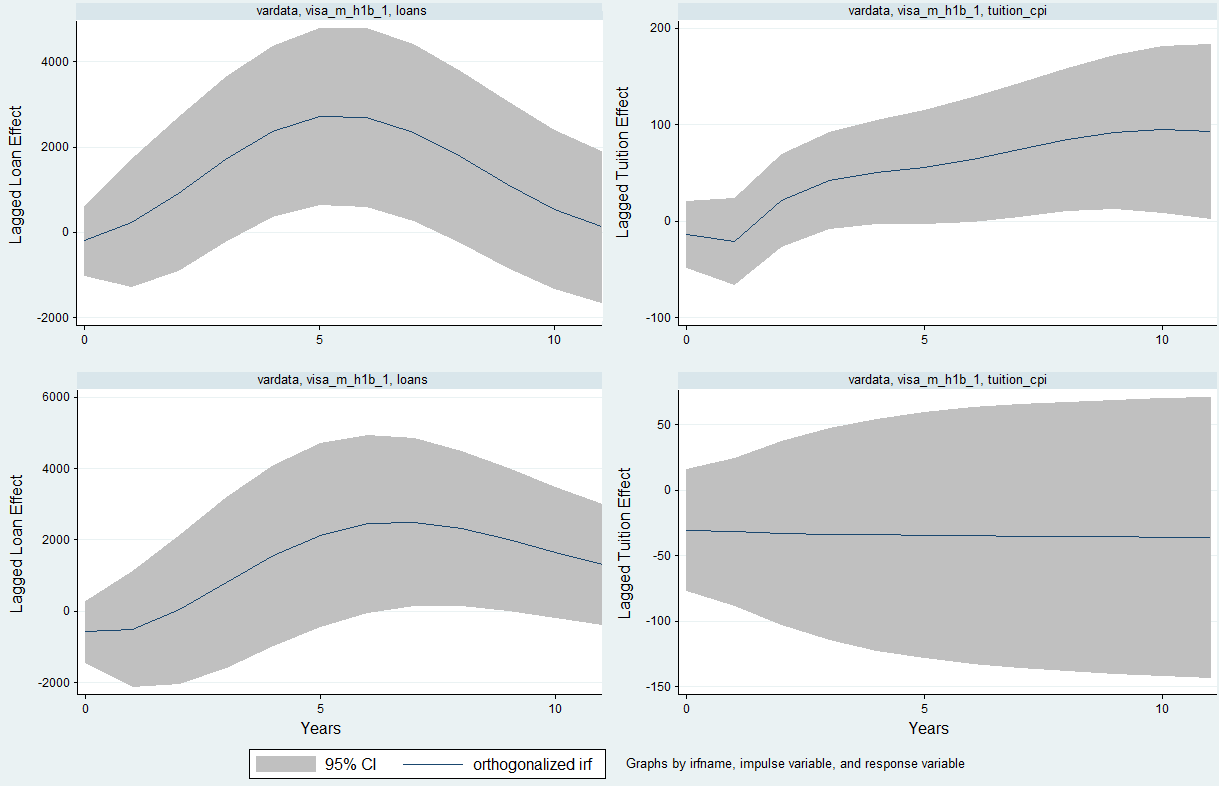
\includegraphics[width=1\textwidth]{./figures-and-tables/fig-1-var-composite.png}};
    \end{tikzpicture}
    \label{fig:var_results}
\end{figure}

Figure \ref{fig:var_results} is a graphical representation of the VAR model results.
The top row contains three-variable models of interest.
In these models, an H-1B impulse generates a first-order enrollment response.
The bottom row contains two-variable specifications that omit the intermediary enrollment response.
On the left are the loan models, and on the right are the tuition models.

The figure makes the three-variable model preference clear for tuition,
but some model statistics make the case stronger with respect to the loan models.
In the two-variable loan VAR, the r-squared for the visa variable is less than 0.89,
and the r-squared for the loan variable is less than 0.988.
In the three-variable specification, the r-squared for the visa variable exceeds 0.913.
The r-squared for the loan variable exceeds 0.989.
This confirms that the enrollment effect is model-improving rather than extraneous complexity.

Both three-variable models achieve significance at the 0.05 level.
SBIC indicates two lag optimization for these models.
The loan model has a sample size of 25 over the years from 1993 to 2017.
The CPI-adjusted tuition model has a sample size of 25 over the years from 1992 to 2016.

The loan model anticipates a temporary increase in total loans, followed by an eventual return to zero.
The tuition model allows for the same, but it also indicates the potential establishment of a new normal
of high real tuition prices.
It does not seem to be the case that a real-world shock would result in one or the other effect.
Instead, a real-world H-1B shock would be expected to cause both effects.
The interaction between loans and higher tuition effects is weak, as previously noted, but it is positively signed.
These models understate the effects of interest if some positive interaction does obtain.

% VAR evidence indicates causality, and granger causality in particular, but I'm not supposed to say that ig...
In summary, vector autoregression provides evidence on H-1B visa issuance as a policy instrument.
H-1B policy stimulus impacts enrollment and has further indirect effects on aggregate student loans and the real price of tuition.
The dynamic response of enrollment and other dependent variables to employer assistance impulse is insignificant.

\section{Conclusions}

% TODO: cleanup begin here

The first goal is to reduce administrative inequities arising from uncertainties.
The second goal is to reduce the complexity
The third policy goal is.

Of note, the CARES act amends Section 127 to temporarily allow the employer tax deduction to apply for the purposes of paying down existing student loan debts.

Logically, critical access issues appear to exist with this implementation.
Solving upward mobility only for those persons who are already employed seems to be a non-starter.
A comparatively better access approach would be to allow anyone to take the deduction.

Two additional access problems exist with those who are employed and have benefit access.
The SHRM report finds that employer assistance is increasingly being used to obtain a graduate degree.


Finally, Lumina Foundation finds that
"only 2-5 percent of eligible employees use tuition assistance programs,
and 43 percent of working adults are unaware if their employer offers such a program."
Finally,

While access problems attenuate the policy effect,
the net effect may be powerful enough to result in a meaningful increase to total enrollment.

Despite logical access problems,
it may be the case that the policy incentive is strong enough to generate a meaningful increase to
In practice, however, many logical effects can add to a negligible practical effect,
motivating the statistical analysis in this paper.


SHRM considers this goal met because Section 127 clarified which expenses can be considered job-related expenses.
SHRM also notes that a prior issue under this policy goal was that
"Entry-level employees, for example, rarely had...legitimate educational assistance paid for by an employer."
The analysis in this paper agrees that Section 127 achieved adminsitrative clarity.
This paper suggests, however, that the clarification created an access issue by restricting legitimate education to accredited education.
This access issue precludes the achievement of certain aspects of the top-level policy goal,
and results in further disadvantage to groups which are already at a disadvantage.

There is another aspect of uncertainty that Section 127 fails to address, which is uncertainty over time.
The initial bill provided for a temporary deduction.
In 2013, an amended bill created a permanent deduction\cite{baldwin_2013}.
This solved the temporal uncertainty problem for a while.
Under the CARES Act, Section 127 was amended to provide a new benefit on a temporary basis\cite{schiavo_2020}.
The new benefit is that employers may assist employees in paying down existing student loan debt,
rather than only paying for new expenses, in a tax deductable way.
It is reasonable to expect such a measure will improve the student loan debt crisis in the United States.
Even so, the measure would be improved according to own policy goals by making the change permanent.

% TODO: cleanup end here

A slowdown in enrollment occurred around the time Section 127 was created.
After thorough correction, the effect of Section 127 remains negative on total enrollment over the period from 1992 to 2016.
The within-period marginal effect of increasing Section 127 assistance is positive.
Vector autoregression does not indicate that this kind of assistance is useful as a policy tool.

This analysis does indicate that the H-1B policy is an important policy tool.
An increase to the count of H-1B visas issued within-period and between periods is associated with increases in enrollment, total loans, and the price of education.
H-1B policy modification in any direction is not obviously beneficial based on these criteria alone.
Legal immigration has several additional benefits that exceed the scope of this study.
The literature generally suggests that an increase in H-1B immigration would benefit the economy\cite{bound2017understanding}.
There are substantial distributional effects, but the net distributional effect appears to be desirable.
The main effects of increased H-1B labor involve a transfer of wealth from native computer scientists to other people,
and other people exhibit significantly higher need on average.

One hypothesis in this paper was that there might be some interaction between H-1B policy and Section 127 assistance.
H-1B policy specifies a college-level education as a qualifier for specialized labor.
Theoretically, this could incentivize higher college participation by natives due to competitive effects.
This study observes no evidence on this kind of effect,
but the removal of the college-level qualifier may still prove beneficial.
Such a move would open the door to a broader pool of talented foreign labor.

Two changes to Section 127 are also worth consideration.
The first change addresses access issues to this deduction.
Willis Towers Watson estimates that fewer than 10 percent of eligible employees use tuition reimbursement benefits annually\cite{merrick_2019}.
Broader Section 127 access is expected to lead to broader utilization.
Additional utilization is expected to improve the significance of the policy effect in an impulse-response specification.

This paper recommends removing the requirement that Section 127 benefit flows through an employer.
A modified Section 127 allows an individual to take a Section 127 deduction for themselves or a dependent.
Allowing dependents to take the deduction reduces the incentive for students to work full-time.
Academic performance suffers for most students that study while working full-time\cite{stamour_2019}.
Allowing an individual to take a deduction without employment would most directly benefit the unemployed.
It would also benefit other groups who tend to be impoverished compared to those currently able to utilize Section 127.
Evidence indicates there exists significant social value due to crime reduction when relatively impoverished individuals obtain a college degree\cite{dennison2019crime}.

% This strategy is similar to the concept of a 529 Plan or an Education Savings Account (ESA),
% but a detailed comparison of these approaches would justify a seperate paper.
% This paper finds no reason to consolidate these policies at this time.

The second recommended change is to allow for the deduction of alternative education costs.
Many employers have ceased requiring the degree in recent years.
Removing the requirement that funds go toward college would reduce upward price pressure on college, and it could incentivize demand for alternative credentials.
Employers prefer alternative credentials for specific roles.
In many cases, obtaining an alternative credential involves a focus on obtaining a specific skill.
A relatively diverse labor pool utilizes these credentials.
Often, these credentials are also more affordable than traditional education.

% Cappelli also provides evidence that employee utilization of educational benefits preferentially go to graduate students.
% This motivates hypotheses on undegraduate access.
% One reason undergraduates might lack access is because they are not being hired.
% Without a job, the undergraduate student is unable to obtain employer assistance.
% This hypothesis motivates theories about why employers began selecting for college graduates.

% Cappelli provides evidence that most employers provide education benefits by 1993,
% The idea that graduate students mainly use employer education benefits motivates hypotheses around undergraduate access.
% Increasingly since the 1990s, developed economies have experienced degree inflation and experience inflation.
% Entry level positions now require a degree when previously this was not necessary, even when technology has made the work easier.
% It is possible that undergraduate access to employer benefits are reduced simply because employers increasingly hire individuals that already have the degree.
% Employers are known to value the degree as a signal of labor quality, but these days there are plenty of other, richer data sources on quality for certain professions.
% In computer programming we see some employers completely dropping the degree requirement and preferring technical interviews, digital portfolio evaluation, and other signals.
% Why, then, do other leading employers continue to require the degree?
% One answer is that the degree requirement forms an H-1B justification.
% Since the passage of the Immigration Act of 1990\cite{law1990law}, a corporation must claim a shortage of qualified specialized labor to justify an H-1B.
% The "attainment of a bachelor's or higher degree" is written into the law as a test of whether labor is qualified and specialized.
% This would motivate employers to begin requiring the degree in order to obtain cheap immigrant labor, even while knowing the degree may not be necessary.
% Such a corrected analysis is exactly what this paper completes.

% we see increasing h-1b increases loans temporarily and tuition permanently, so it's bad right? not so fast!
% h-1b labor is specialized immigrant labor, so it's beneficial for the economy. Maybe even net of above negative impacts.
% what if we could get all of the benefit of immigration without the cost of loans and tuition, credential inflation, etc?
% potential solution: change H-1B to remove the degree as meaningful. Employers are already throwing it out!
% use alternative credentials. alternative learning is adaptive and effective, cheaper and super cool. even resistant to COVID!
% the total effect of assistance in the relevant range is positive, and additional real assistance would further boost attendance.
% however, it's not obvious that increased attendance is a good thing. credential inflation, experience inflation, debt crisis.
% i fail to find evidence supporting a significant interaction between section 127 and visa policy
% however visa policy in itself is extremely important in the conversation on enrollment, credential inflation, experience inflation, and debt crisis.
% there are important caveats in this visa analysis.
% employers have recently been removing the degree requirement
% the law should also remove that requirement and boost alternative education which doesn't require a formal degree and is highly effective
% this will reduce debt, improve diversity and economic efficiency and individual skill

% 75 percentile for salaries in 2017 was 54250 https://bizfluent.com/info-10032733-percentile-salary.html
% define middle class as 50-75 percentile, lower class as under 50 percentile. break down effect by salary classification and see if it helps lower/middle
% if so, it should improve diversity of education leading to a more diverse workforce which employers crave (TM) and politicians, etc...
% Should we actually enact this policy? Effect on alternative credentials and credential inflation
% Other options like extending the benefit to repayment https://blog.shrm.org/blog/let-s-fight-the-skills-gap-by-expanding-tax-free-education-assistance
% we can also consider extending the education benefit to unaccredited education and income share agreements not just loans

% https://www.nber.org/papers/w9225.pdf 
% https://www.nber.org/digest/feb03/w9225.html

\bibliography{./BibFile}

\end{document}
